\documentclass[a4paper,12pt]{article}
\usepackage[utf8x]{inputenc}
\usepackage[spanish]{babel}
\usepackage{amsmath}
\usepackage{graphicx}
\setlength{\textheight}{235mm}
\setlength{\textwidth}{168mm}
\setlength{\oddsidemargin}{0pt}
\pagestyle{empty}

\begin{document}
\mbox{}\vspace*{-45mm}

{\centering
{\small\sc Escuela Técnica Superior de Ingenieros de Caminos, Canales y
Puertos (Madrid)}\\*[4mm]
{\Large\bf Método de los Elementos Finitos}\\*[4mm]
PRÁCTICA 4: Modelos de difusión \\*[4mm]
}

\vspace{3mm}

\parbox{70mm}{ 
Se considera una chapa cuyas dimensiones y geometría son las indicadas
en la figura adjunta. Los lados de la chapa tienen condiciones de contorno 
correspondientes a temperaturas o flujos impuestos, cuyos valores
también están indicados en dicha figura. Los bordes en los que no se indica
el flujo o la temperatura impuesta se supone que están térmicamente aislados.
El coeficiente de conductividad térmica es $\lambda=380$ W/(m$\cdot$K).

Se desea conocer la distribución de temperaturas y el flujo de calor en la
chapa.
} \hfill
\parbox{80mm}{
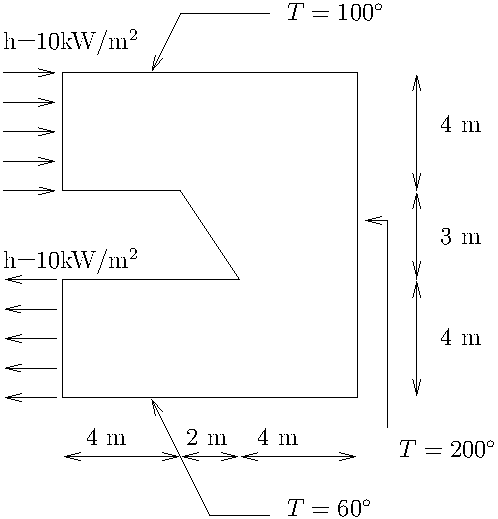
\includegraphics{practi4}
}

\end{document}
